\documentclass[a4paper,11pt]{article}
\usepackage{amsmath} 
\usepackage{amsfonts}
\usepackage{graphicx}
\usepackage{algorithm,algorithmic}
\usepackage{url}
\usepackage{color}
\usepackage{tikz}
\usepackage{multirow}
\usepackage{verbatim}
\usepackage{hyperref}
\usepackage{float}
\usepackage{geometry}
\usepackage{indentfirst}
\usepackage{amssymb}

%\usepackage{draftwatermark}
\usepackage{listings}
\usepackage{makeidx}

\usepackage{times}


\usepackage{longtable}

\geometry{left=3.17cm,right=3.17cm,top=2.54cm,bottom=2.54cm}
%\begin{comment}
\pagestyle{empty}
%\end{comment}
\begin{document}
\begin{center}
{\large Documentation for the OPAL Boundary Geometry Features} \\
Chuan Wang, Andreas Adelmann \\
\today\\
\end{center}
\section{Introduction}
The boundary geometry feature of OPAL \cite{OP} provides complex geometry handling capabilities for dark current and multipacting simulations. The boundary geometry features includes the following aspects:
\begin{enumerate}
\item particle-boundary collision test 
\item boundary surface physics model including field emission and secondary emission
\item input, output and visualization of geometry model.
\end{enumerate}
\section{Particle-boundary collision test model}
A crucial part is efficient detection of a collision of a particle with, a possiible complex, surrounding boundary. 
\subsection{Basic idea: line segment-triangle intersection test}
The particle-boundary collision test in a 3D geometry is complicated, because the geometry is hard to be parameterized by simple functions like in the 2D case. A more practical way is to use a triangulated surface mesh to represent complicated 3D geometry. So 3D line segment-triangle intersection (LSTI) tests are needed. There already efficient algorithms exist for LSTI test \cite{FA} without precomputing. Here, as we need triangle normal for later physics model computation, an algorithm faster but using precomputed normal is adopted \cite{LT}. The input parameters of this algorithm are the starting point and end point of the line segment, vertices and normal of the triangle, as sketched in Figure \ref{fig:L-T}. Here $\vec{n}$, $\vec{u}$, $\vec{v}$ and  $\vec{w}$ are vectors, and points are in 3D space, i.e., $\mathbf{x}_0,\mathbf{x}_1,\mathbf{t}_0,\mathbf{t}_1,\mathbf{t}_2,\mathbf{I} \in \mathbb{R}^3$. Other symbols in Figure \ref{fig:L-T} are scalars.  \\
\begin{figure}[H]
\begin{center}
\scalebox{0.7}{
\begin{tikzpicture}
\usetikzlibrary{arrows}
\draw [->,black,-latex] (-1.5,0) -- (1.5,0);
\draw [->,black,-latex] (-1.5,0) -- (-1.5,2);
\draw (1.5,0) -- (0.0,2);
\draw  [<-,black,latex-](0.0,2) -- (-1.5,0.0);
\draw [->,black,-latex,dashed] (-1.5,0) -- (0.5,0.5);
\node[below] (w) at (-0.15,0.5) {$\vec{w}$};
\draw[dashed] (0.5,0.5) -- (-1.18,0.5);
\draw[dashed] (0.5,0.5) -- (0.01,0.0);
\node[above] (ti) at (-1.18,0.5) {$t_i$};
\node[below] (si) at (0.01,0.0) {$s_i$};
\node[above] (t0) at (-1.7,0.) {$\mathbf{t_0}$};
\node[right] (t1) at (1.5,0) {$\mathbf{t_1}$};
\node[above] (t2) at (0.0,2.0) {$\mathbf{t_2}$};
\node[above] (n) at (-1.5,2) {$\vec{n}$};
\node[above] (v) at (-0.5,1.5) {$\vec{v}$};
\node[below] (u) at (1.2,0.0) {$\vec{u}$};
\path[draw=black,fill=black] (0.0,2.0) circle (2pt);
\path[draw=black,fill=black] (1.5,0.0) circle (2pt);
\path[draw=black,fill=black] (-1.5,0.0) circle (2pt);
\draw (-3.5,-1) -- (2.5,-1);
\draw (2.5,-1) -- (5,3);
\draw (0,3) -- (5,3);
\draw (-3.5,-1) -- (0,3);
\draw (0.5,0.5) -- (1.6,5);
\path[draw=black] (0.5,0.5) circle (2pt);
\node[above] (I) at (0.5,0.5) {$\mathbf{I}$};
\node[right] (x0) at (1.6,5) {$\mathbf{x_0}$};
\draw[dashed] (0.5,0.5) -- (-0.1,-1.9);
\node[right] (x1) at (0.0,-1.9) {$\mathbf{x_1}$};
\node[right] (ri) at (1,2.5) {$r_i$};
\path[draw=black,fill=black] (-0.1,-1.9) circle (2pt);
\path[draw=black,fill=black] (1.6,5) circle (2pt);
\end{tikzpicture}
}
\end{center}
\caption{Line segment-triangle intersection()\label{fig:L-T}}
\end{figure}
The basic algorithm is as follows:
\begin{algorithm}[H]
   \caption{Line Segment- Triangle Intersection Algorithm} \label{alg:mg_algo}
   \begin{algorithmic}[1]
     \STATE \textbf{procedure} LSTI (In: line segment $\mathbf{x}_1-\mathbf{x}_0$, $\Delta(\mathbf{t}_0, \mathbf{t}_1, \mathbf{t}_2)$ Out: true $ \&\ \mathbf{I}$ or false)

     \IF{$\vec{n} \cdot (\mathbf{x}_1-\mathbf{x}_0)=0$}
     \RETURN false ($\mathbf{x}_1-\mathbf{x}_0~||~\Delta \rightarrow$ no intersection)
     \ELSE
     \STATE $ r_i=\frac{\vec{n} \cdot (\mathbf{t}_0-\mathbf{x}_0)}{ \vec{n}\cdot(\mathbf{x}_1-\mathbf{x}_0)} $
     \STATE The intersection point of the line segment and plane: $ \mathbf{I}=\mathbf{x}_0+r_i(\mathbf{x}_1-\mathbf{x}_0) $ 
     \IF{$ r_i $$<$$ 0$ or $ r_i$ $>$ $1 $}
     \STATE Do early rejection as intersection is on the extension of line segment 
     \ELSE 
     \STATE (Check if the intersection point is inside the triangle)
     \STATE The parametric plane equation: $ \mathbf{t}(s_i,t_i)=\mathbf{t}_0+s_i (\mathbf{t}_1-\mathbf{t}_0)+t_i(\mathbf{t}_2-\mathbf{t}_0)=\mathbf{t}_0+s_i\vec{u}+t_i\vec{v} $. As $\vec{w}=\mathbf{I}-\mathbf{t}_0$ is also in the plane, solve equation: $\vec{w}=\mathbf{t}_0+s_i\vec{u}+t_i\vec{v}$ 
     \STATE $ s_i=\frac{(\vec{u} \cdot \vec{v})(\vec{w} \cdot \vec{v})-(\vec{v} \cdot \vec{v})(\vec{w} \cdot \vec{u})}{(\vec{u} \cdot \vec{v})^2-(\vec{u} \cdot \vec{u})(\vec{v} \cdot \vec{v})} $,  $ t_i=\frac{(\vec{u} \cdot \vec{v})(\vec{w} \cdot \vec{u})-(\vec{u} \cdot \vec{u})(\vec{w} \cdot \vec{v})}{(\vec{u} \cdot \vec{v})^2-(\vec{u} \cdot \vec{u})(\vec{v} \cdot \vec{v})} $.
     \IF{$ s_i \geq 0 $, and $ t_i \geq 0 $ and $ s_i+t_i \leq 1 $} 
     \STATE The intersection is inside the triangle, and return the intersection points.
     \ELSE
     \RETURN false (no intersection between the line segment and the triangle)
     \ENDIF
     \ENDIF
\ENDIF
       \STATE \textbf{end procedure}
   \end{algorithmic}
 \end{algorithm}
The parameters and symbols used in the above algorithm are the same with those in Figure \ref{fig:L-T}. 
% 1)find the intersection between line segment $ \vec{x1-x0} $ and plane defined by point t0 and triangle normal. If the dot product of line segment and plane normal equals to zero and x0 is not the barycentric point of the triangle(in the plane), then the line segment is parallel to plane return no intersection, else if the particle is really move ($ x0 \neq x1 $),return initialized position-triangle barycentric point as intersection.The intersection position rI w.r.t x0 is obtained from: $ rI=\frac{\vec{n} \cdot \vec{(t0-x0)}}{\vec{n} \cdot \vec{(x1-x0)}} $,where t0 is the first vertex of triangle, n is the normal of triangle. The intersection point Itsec is obtained from: $ Itsec=x0+rI(x1-x0) $. \\
% 2)Check if the intersection point is inside the triangle by using parametric coordinates sI and tI of the intersection point. First calculate sI and tI. The parametric plane equation is given by:  $ t(sI,tI)=t0+sI(t1-t0)+tI(t2-t0)=t0+sI\vec{u}+tI\vec{v} $.$\vec{w}=\vec{Itsec-t0}$ is also in the plane, solve equation: $\vec{w}=t0+sI\vec{u}+tI\vec{v}$ , we obtain the sI and tI. $ sI=\frac{(\vec{u} \cdot \vec{v})(\vec{w} \cdot \vec{v})-(\vec{v} \cdot \vec{v})(\vec{w} \cdot \vec{u})}{(\vec{u} \cdot \vec{v})^2-(\vec{u} \cdot \vec{u})(\vec{v} \cdot \vec{v})} $, $ tI=\frac{(\vec{u} \cdot \vec{v})(\vec{w} \cdot \vec{u})-(\vec{u} \cdot \vec{u})(\vec{w} \cdot \vec{v})}{(\vec{u} \cdot \vec{v})^2-(\vec{u} \cdot \vec{u})(\vec{v} \cdot \vec{v})} $. If $ sI \geq 0 $, $ tI \geq 0 $ and $ sI+tI \leq 1 $, then the intersection is inside the triangle, and return the intersection coordinate Itsec.\\
\subsection{Early rejection strategy}
Although the faster algorithm using precomputed triangle normal is implemented, the line segment-triangle test still could be time consuming. Effective early rejection strategy is needed to reduce the number of LSTI test. The basic schemes of our strategy are as in Figure~\ref{fig:P-B}.
\begin{figure}[H]
\begin{center}
/Users/adelmann/svnwork/adelmann/papers/figures/Latex-Figures/2d_grid.tikz
\end{center}
\caption{Schematic view of particle-boundary hitting test.\label{fig:P-B}}
\end{figure}
The dark black curve, the colored circles, the dashed grids, the dark black arrow,  and the light gray arrow in Figure \ref{fig:P-B} stand for boundary surface, simulated particles, axis aligned space partition boxes, the momenta of particle, and boundary inward normal $\vec{n}$ respectively.\\

Assuming we need to determine whether a particle with position $\mathbf{r}$ and momenta $\mathbf{v}$ will hit the boundary within time step $\Delta{t}$.\\ 

We first test if the particle is near the boundary by checking if $\mathbf{r}$ is inside the boundary bounding boxes which are illustrated by gray grids in Figure ~\ref{fig:P-B}. If $\mathbf{r}$ is not in bounding box as the green particle case in Figure ~\ref{fig:P-B}, the particle is far from boundary and will be integrated directly without accurate line segment-triangle intersection test. If $\mathbf{r}$ is in bounding box like the yellow particle and the red particle cases in Figure ~\ref{fig:P-B}, then traversal all the triangles in the bounding cubic box which the particle is in, as well as triangles in the adjacent 26 bounding cubic boxes, to see if the momenta of the particle has opposite direction with those triangles' normals. If it is not true like the yellow one, do integration without line segment-triangle intersection test. If it is true like the red one, then check if the particle has intersection with those triangles by doing LSTI test. If intersection exists,  particle will hit the boundary during the current time step. \\

Two things need to be point out. First one is that we get inward normal in the following way. We find a point close to a triangle with ID number equals to 1, and determine the point is inside or outside the boundary geometry by doing ray-boundary intersection test and count the number of intersections. Using this point we can get the orientation(inward normal) of triangle 1. Then we can get the inward normal of all surface triangles by recursively aligning the orientation of adjacent triangles of those triangles whose inward normals have already obtained. The second one is that the success of the above particle-boundary collision test lies on the fact that the length that particles travel in one time step is no larger than the bounding box size, i.e, the particle will not cross the bounding box within one time step.\\
\section{Boundary surface physics model}
\subsection{Field emission model}
Field emission is crucial to dark current and is a major source of primary incident particles in secondary emission. The Fowler-Nordheim (F-N) formula we use here to predict the emitted current density is as follows \cite{BC} \cite{FN}\\

\begin{equation*}
%J(r,t) = 1.54\times10^{(-6+\frac{4.52}{\sqrt{\varphi}})}\frac{(\beta E)^2}{\varphi}\exp{(\frac{-6.53\times10^9\varphi^{1.5}}{\beta E})}
J(\mathbf{r},t) = \frac{A(\beta E)^2}{\varphi t(y)^2}\exp{(\frac{-B v(y)\varphi^{3/2}}{\beta E})},
\end{equation*}
where $J(\mathbf{r},t)$ stands for emitted electric current density in position $\mathbf{r}$ and time $t$. The Greek letters $\varphi$ and  $\beta$ are the work function of surface material and the local field enhancement factor respectively. The parameter $E$ is the electric field in the normal direction of surface. The parameters $A$ and $B$ are empirical constants. The functions $v(y)$ and $t(y)$ representing the image charge effects \cite{BC} are the function of the Fowler-Nordheim parameter $y$ which has the definition\cite{DE}:\\
\begin{equation*}
y = \sqrt{\frac{e^3}{4\pi\varepsilon}}\frac{\sqrt{\beta E}}{\varphi} = 3.795\times10^{-5}\frac{\sqrt{\beta E}}{\varphi}.
\end{equation*}
Here, we choose a simpler approximation \cite{DE} $v(y)=a-by^2$ and $t(y)\approx 1$. These approximations will be valid for a large range of $y$ , which correspond to typical applied electric field range in RF guns.\\   

We have some user defined parameters in OPAL Distribution class for user to handle their own field emission simulation. The name, default value, unit and meaning of those parameters for dark current are summarized in Table \ref{table:nonlin}.\\

\begin{table}[H]
\small
\caption{User defined parameters for dark current and field emission} % title of Table
\centering % used for centering table 
\begin{tabular}{lccc} % centered columns (4 columns)

 
\hline\hline %inserts double horizontal lines
Name & Default value & Unit & Meaning \\ [0.5ex] % inserts table 
%heading 
\hline % inserts single horizontal line
NPDARKCUR & 1000.0 & - & No. of randomly initialized dark current electrons\\ % inserting body of the table
INWARDMARGIN & 0.001 & m & Inward margin of initialized dark current electrons\\
FNA & $1.54\times10^{-6}$ & - & Empirical constant A for F-N emission model\\
FNB & $6.83\times10^9$ & - & Empirical constant B for F-N emission model \\
FNY & $3.795\times10^{-5}$ & - & Constant for image charge effect parameter y(E) \\ [1ex]% [1ex] adds vertical space
 &  &  & ( Use default value of FNY for electrons) \\
FNVYZERO & $0.9632$ & - & Zero order constant for v(y) function \\
FNVYSECOND & $1.065$ & - & Second order constant for v(y) function \\ 
FNPHIW & $4.65$ & eV & Work function of gun surface material \\ 
FNBETA & $50.0$ & - & Field enhancement factor $\beta$ for F-N emission \\
FNFIELDTHR & $30.0$ & MV/m & Field threshold for F-N emission \\
FNMAXEMI & $20.0$ & - & Max. No. of electrons emitted from a single triangle \\
\hline %inserts single line 
\end{tabular} 
\label{table:nonlin} % is used to refer this table in the text 
\end{table}

Also, as our space charge solver for complicated boundary geometry is not finished yet, we simply take the 1D Child-Langmuir law into our field emission model to represent the space charge limited field emission. This is not the exact situation in the real field emission with space charge limited current density, as is shown by 1D simulation \cite{BC}. But it will be closer to the real situation. The 1D Child-Langmuir law is: \\ 
\begin{align*}
J(\mathbf{r},t) & =\frac{4\varepsilon_0}{9}\sqrt{2\frac{e}{m}}(\frac{V^{3/2}}{d^2})\\
 & =\frac{4\varepsilon_0}{9}\sqrt{2\frac{e}{m}}(\frac{E^{3/2}}{d^{1/2}})
\end{align*}
 where $J(\mathbf{r},t)$ is space charge limited emission current density in position $\mathbf{r}$ and time $t$, $\varepsilon_0$ is permittivity in vacuum, $E$ is the normal component of electric field in surface, $d$ is the distance from the position where $E$ is evaluated. Currently we choose $d$ equals the length that emitted particles move in one time step, i.e., $d=\frac{eE\Delta{t}^2}{2m_0}$ where $\Delta{t}$ is simulation time step.\\ 

In each time step for each surface triangle with field emission tag, we compare the emitted current predicted by F-N formula and Child-Langmuir law, and if the previous value is larger then the space charge may not be ignored, and we use Child-Langmuir law to calculate the emitted particle number. If the emitted number exceed the maximum number defined by user in FNMAXEMI, the emitted particle number will be set to equal to the FNMAXEMI, and the charge per emitted particle will be multiplied by a scaling factor defined by: calculated emitted particle number $/$ FNMAXEMI.\\   

\subsection{Secondary emission model}

Our secondary emission module is based on a phenomenological model developed by M. A. Furman and M. Pivi\cite{SE}. This module calculates the number of secondary electrons that
result from an incident electrons of a given energy on a material
at a given angle (see Figure~\ref{incident electrons}). For each of
the generated secondary electrons the associated process: {\em true secondary}, {\em rediffused} or
{\em back scattered} is recorded in the variable {\it seType}. 

\begin{figure}[H]
\centering
\scalebox{0.7} {
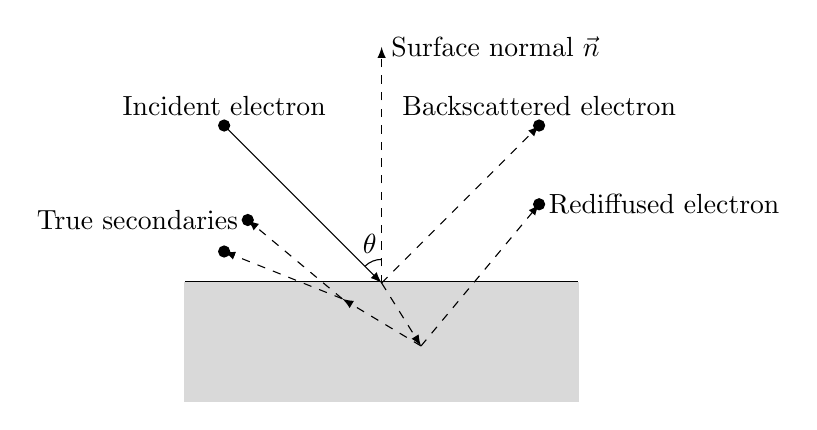
\begin{tikzpicture}
\usetikzlibrary{arrows}
\draw [very thick] (-2.5,0) -- (2.5,0);
\draw[gray!30,fill=gray!30] (-2.5,-1.5) rectangle (2.5,0); 
\draw [->,dashed,-latex] (0,0) -- (0,3);
%\node[below] (w) at (-0.15,0.5) {$\vec{w}$};
\node[right] (n) at (0,3) {Surface normal $\vec{n}$};
\path[draw=black,fill=black] (-2,2.0) circle (2pt);
\node[above] (electron) at (-2,2) {Incident electron};
\path[draw=black,fill=black] (2,2.0) circle (2pt);
\node[above] (electron1) at (2,2) {Backscattered electron};
\draw [->,-latex] (-2,2.0) -- (0,0);
\draw [dashed,->,-latex]  (0,0) -- (2,2.0);
\draw [dashed,->,-latex]  (0,0) -- (0.5,-0.8);
\draw [dashed,->,-latex]  (0.5,-0.8) -- (2,1);
\path[draw=black,fill=black] (2,1.0) circle (2pt);
\node[right] (electron1) at (2,1) {Rediffused electron};
\draw [dashed,->,-latex]  (0.5,-0.8) -- (-0.5,-0.2);
\draw [dashed,->,-latex] (-0.5,-0.2) -- (-2,0.4);
\draw [dashed,->,-latex] (-0.5,-0.2) -- (-1.7,0.8);
\path[draw=black,fill=black] (-2,0.4) circle (2pt);
\path[draw=black,fill=black] (-1.7,0.8) circle (2pt);
\node[left] (electron1) at (-1.7,0.8) {True secondaries};
\node[above] (theta) at (-0.15,0.25) {$\theta$};
\draw (0,0.3) arc (90:135:0.3);
\end{tikzpicture}
}
% \includegraphics[width=3 in]{incident_diagram.pdf}
\caption{Geometry used by the secondary electrons module}
\label{incident electrons}
\end{figure}


The prototype for the function used in our secondary module is described in Listing 1. 

%The return values of normalized velocity (bn,bt,bz) must be arrays of size 10.  

\begin{verbatim}
void nSec(const double &incEnergy,  const double &cosTheta, 
          const int &matNumber, int &seNum, int &seType, 
          const double &incQ, const Vector_t &TriNorm, 
          const Vector_t &inteCoords, const Vector_t &localX, 
          PartBunch *itsBunch) 
\end{verbatim}

Table \ref{nsec.table} describes the parameters for nsec.
Note that the final four parameters are filled in by the function itself
and used as return values.

\begin{centering}
\begin{longtable}{|l|p{4in}|}
\caption{nsec --- parameters\label{nsec.table}} \\
\endfirsthead

\multicolumn{2}{c}
{{\bfseries \tablename\ \thetable{} -- continued from previous page}} \\
\hline
Parameter	& Description											\\
\hline
\endhead

\hline \multicolumn{2}{r}{{Continued on next page}} \\ \hline

\endfoot

\hline
\endlastfoot

\hline
incEnergy	& energy of incident electrons expressed in eV	 \\
cosTheta	& the angle of incidence expressed at the cosine of the angle measured with 0 as normal (costheta = 1 at normal incidence) \\
matNumber	& the material being struck by the incident electrons (0 = copper, 1 = stainless steel)	\\
\hline
seNum			& number of secondary electrons	\\
seType			& type of secondary electrons (2=true secondary, 1=rediffused, 0=back scattered) \\

incQ			& charge of incident electrons \\
TriNorm			& inward normal of surface triangle	\\
inteCoords		& incident position			\\
localX                 & coordinates of a point to define the x axis of local coordinate\\
itsBunch                & pointer to OPAL particle bunch object used for generating secondaries\\
\hline
\end{longtable}

\end{centering}
In particle tracking module of OPAL, i.e., the ParallTTracker class, we use Boris pushing scheme to push particles in each time step. We do particle-boundary collision test after particles have got new external field, new self-field, new momentum and consequently new position in the end of each time step for non secondary case.\\

For secondary emission simulation in OPAL, we need to do two additional collision tests on newly generated secondaries before pushing them in the first half and second half of each step, as they have non zero initial momentum and thus have non zero possibility to collide the boundary during pushing. \\ 



\begin{thebibliography}{99}
\bibitem{OP} A. Adelmann and Ch. Kraus and Y. Ineichen and  J. Yang,
The OPAL (Object Oriented Parallel Accelerator Library) 
              Framework, Paul Scherrer Institute, PSI-PR-08-02, 2008
\bibitem{FA} T. M\"oller and B. Trumbore,
 ACM SIGGRAPH 2005 Courses, July 31-August 04, 2005, Los Angeles, California   [doi:10.1145/1198555.1198746] 
\bibitem{LT} D. Sunday,
 available online on:\\ \href{http://softsurfer.com/Archive/algorithm\_0105/algorithm\_0105.htm}{http://softsurfer.com/Archive/algorithm\_0105/algorithm\_0105.htm}
\bibitem{BC} Y. Feng and J. P. Verboncoeur,
Phys.Plasmas 13, 073105 (2006)
\bibitem{FN} R. H. Fowler and L. Nordheim, 
Proc. R. Soc. London, Ser. A 119, 173 (1928)
\bibitem{DE} J. H. Han, PhD Thesis, Desy, 2005 available online on \href{http://www-library.desy.de/preparch/desy/thesis/desy-thesis-05-045.pdf}{http://www-library.desy.de/preparch/desy/thesis/desy-thesis-05-045.pdf}
\bibitem{SE} M. A. Furman and M. Pivi, 
 Phys. Rev. ST Accel. Beams 5, 124404 (2002)
\end{thebibliography} 
\end{document}

